\begin{frame}
        \titlepage
\end{frame}

\begin{frame}[t]
    \frametitle{Overarching goal}

    We want to study the separation behavior of polymers.

    \vfill

    \begin{columns}
        \begin{column}{0.6\textwidth}
            \begin{itemize}
                \item \onslide<2-> A \emph{polymer} is a large molecule, composed of many repeated subunits (\emph{monomers}, smaller molecules).
                \item \onslide<3-> Momoners interact with each other in and across polymers.
                \item \onslide<4-> Simplest kinds of polymers are of linear chain type.
                \item Stochastic models (e.g. random walks, ideal chain models) are used to model these.
            \end{itemize}
        \end{column}
        \begin{column}{0.4\textwidth}
            \centering
            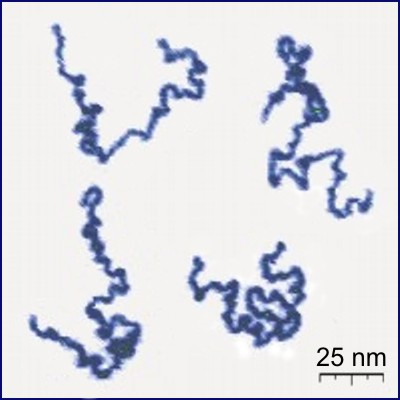
\includegraphics[width=0.9\textwidth]{figures/Single_Polymer_Chains_AFM.jpg}
        \end{column}
    \end{columns}
\end{frame}

\begin{frame}[t]
    \frametitle{Overarching goal}

    \vfill

    \begin{itemize}
        \item Polymer melts (liquid phase) can exhibit different separation behaviors:
        \onslide<2->
        \begin{itemize}
            \item \emph{macrophase separation:} liquid-liquid separation (e.g. like water / oil); mostly seen in blends of different polymers.
            \item \emph{microphase separation:} distinct ordering of individual polymer chains.
        \end{itemize}
        \onslide<3->
        \item We are interested in the microphase separation of \emph{diblock copolymers}.
        \item These consist of two types of monomers (e.g. A and B) forming two large blocks.
    \end{itemize}

    \centering
    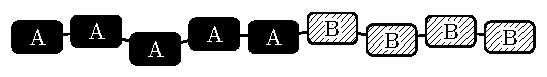
\includegraphics[width=0.8\textwidth]{figures/copoly2.pdf}
\end{frame}

\begin{frame}[t]
    \frametitle{Overarching goal}

    Several types of microphase separation observable depending on the properties of the polymers, e.g. gyroid:

    \centering
    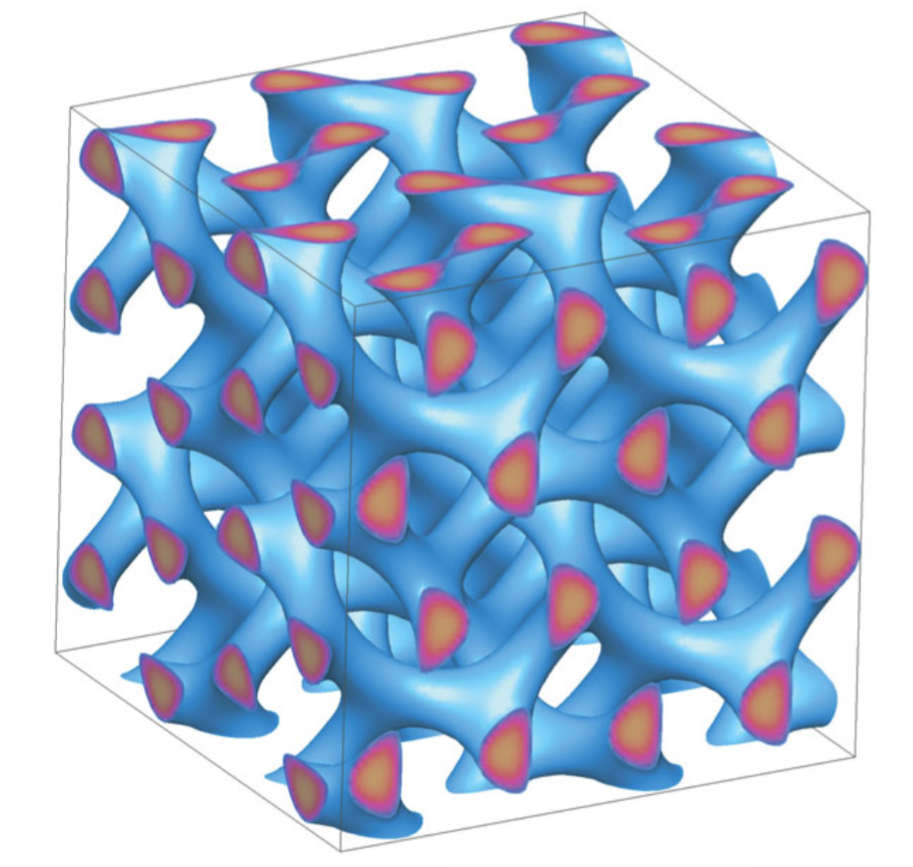
\includegraphics[scale=0.15]{figures/gyroid_separation.png}

    \onslide<2->
    So how can we predict the microphase separation of polymers through theoretical models?
\end{frame}

\begin{frame}[t]
    \frametitle{So, what's self-consistent field theory?}

    Self-consistent field theory (scft) allows us to study the behavior of large stochastic models through simplified models.

    \vfill
    \begin{itemize}
        \item \onslide<2-> \emph{Goal:} study a complex stochastic model (e.g. a polymer melt) with a huge number of small individual interacting components (e.g. monomers).
        \item \onslide<3-> \emph{Idea:} instead of considering interactions between all the individual components, approximate the effect on a given individual by a single averaged effect (so called \emph{external field}).
    \end{itemize}

    \vfill
    \centering
    \onslide<4->
    \emph{This reduces a many-body problem to a one-body problem!}
\end{frame}

\begin{frame}[t]
    \frametitle{So, what's self-consistent field theory?}

    How can this be used?


    \begin{itemize}
        \item Model leads to a free energy functional depending on external fields $w_{A}$ and $w_{B}$, where saddle points correspond to stable microphase separations!
        \item \onslide<2-> Allows an iterative scheme that adjusts the external fields until these satisfy some saddle point equations (\emph{self consistency}).
    \end{itemize}
\end{frame}

\begin{frame}[t]
    \frametitle{So, what's self-consistent field theory?}

    Most costly part of one iteration:
    calculating a solution to the modified diffusion equation (mde)
        \begin{equation}
            \frac{\partial}{\partial s}q(\vec{r}, s) = \Delta q(\vec{r}, s) - w(\vec{r}, s)q(\vec{r}, s), \quad q(\vec{r}, 0) = 1,
        \end{equation}
    with
    \begin{itemize}
        \item the normalized polymer chain contour $s \in [0, 1]$,
        \item a position in a small volume cell $\vec{r}$,
        \item the combined external field
        \begin{equation}
            w(\vec{r}, s) = \begin{cases}
                w_{A}(\vec{r}), & 1 \leq s < f \\
                w_{B}(\vec{r}), & f < s \leq 1
            \end{cases}
        \end{equation}
        with the proportion $f \in [0, 1]$ of $A$-type monomers in the polymer chain.
    \end{itemize}
\end{frame}

\begin{frame}[t]
    \frametitle{So, what's self-consistent field theory?}

    \vfill

    \begin{itemize}
        \item Mde has to be solved several hundred / thousand times with slight variations in the external fields.
        \item \onslide<2-> Some kind of model reduction resulting in a speed up of the iterative scheme would be useful!
    \end{itemize}

    \vfill
    \onslide<3->
    Let's look at some examples that can be obtained by the iterative scheme in the case of one spatial dimension
    (using a de facto default pseudospectral method for the mde).
    \vfill
\end{frame}

\begin{frame}[t]
    \frametitle{Example}

    \begin{itemize}
        \item Let $f = 1/2$.
        \item \uncover<2->{On the left: the final fields $w_A$ and $w_B$.}
        \item \uncover<3->{On the right: the corresponding fourier coefficients (in the order $\cos(2 \pi), \sin(2 \pi), \cos(4 \pi), \dots$).}
    \end{itemize}

    \vfill
    \begin{columns}
    \begin{column}{0.5\textwidth}
        \uncover<2->{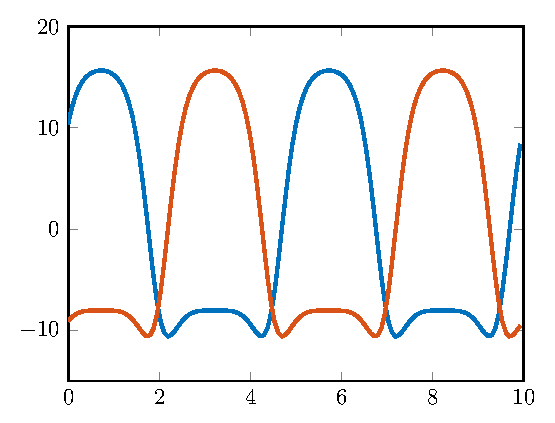
\includegraphics[width=\textwidth]{figures/scft1.pdf}}
    \end{column}
    \begin{column}{0.5\textwidth}
        \uncover<3->{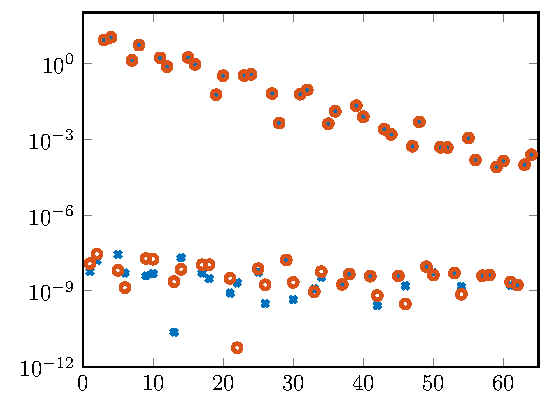
\includegraphics[width=\textwidth]{figures/scft2.pdf}}
    \end{column}
    \end{columns}
\end{frame}

\begin{frame}[t]
    \frametitle{Example}

    And now the same with $f = 1/3$.

    \vfill
    \begin{columns}
    \begin{column}{0.5\textwidth}
        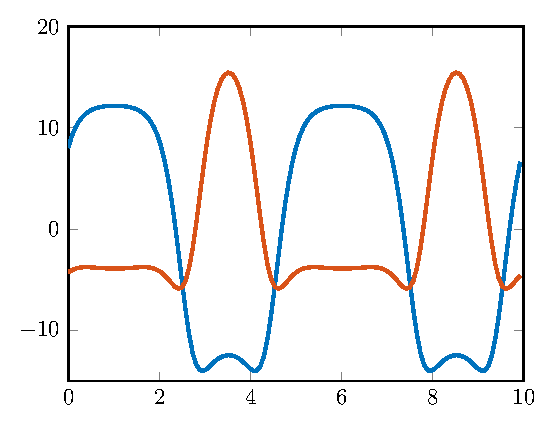
\includegraphics[width=\textwidth]{figures/scft_example2_fields.pdf}
    \end{column}
    \begin{column}{0.5\textwidth}
        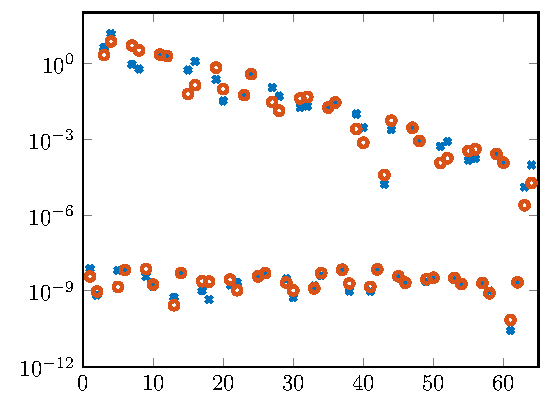
\includegraphics[width=\textwidth]{figures/scft_example2_fourier_coeffs.pdf}
    \end{column}
    \end{columns}
\end{frame}

\begin{frame}[t]
    \frametitle{What's striking?}

    \begin{itemize}
        \item External fields exhibit regularity and some kind of symmetry.
    \end{itemize}

    \vfill

    \begin{columns}
        \begin{column}{0.5\textwidth}
            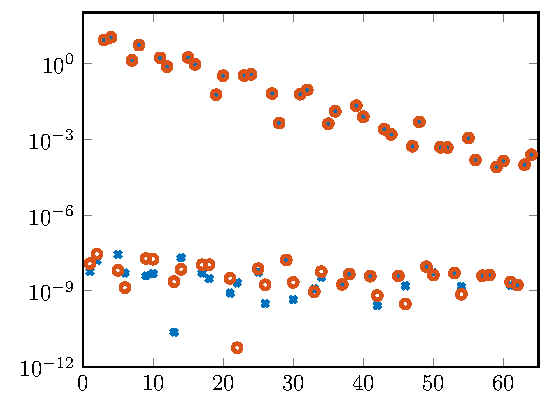
\includegraphics[width=\textwidth]{figures/scft2.pdf}
        \end{column}
        \begin{column}{0.5\textwidth}
            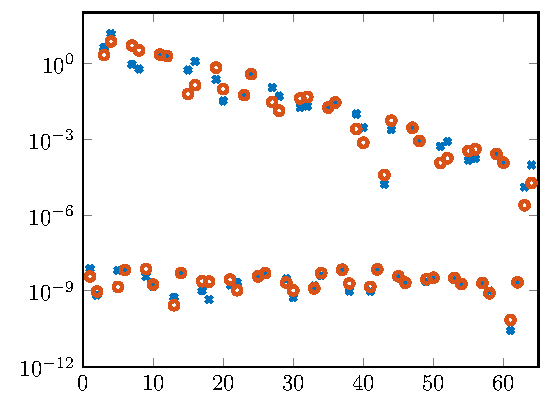
\includegraphics[width=\textwidth]{figures/scft_example2_fourier_coeffs.pdf}
        \end{column}
    \end{columns}

    \onslide<2->
    Maybe this can be used as a leverage point for a model reduction by only considering the functions with significant coefficients
    $\rightarrow$ Reduced basis method.
\end{frame}

\begin{frame}[t]
    \frametitle{Intermission: Reduced Basis Method}
    \framesubtitle{Preliminaries}

    Given a parametric variational problem
    \begin{equation}
        b(u, v; \bm \sigma) = f(v), \qquad u \in \mathcal X, v \in \mathcal Y,
    \end{equation}
    where
    \begin{itemize}
        \item $\mathcal X, \mathcal Y$ are Hilbert spaces,
        \item $\mathcal P \subset \mathbb{R}^{P}$, $P \in \mathbb{N}$, is a closed parameter space,
        \item $b \colon \mathcal X \times \mathcal Y \times \mathcal P \to \mathbb{R}$ is a parametric continuous bilinear form,
        \item $f \colon \mathcal Y \to \mathbb{R}$ is a continuous linear functional.
    \end{itemize}

    \onslide<2->
    Let's assume we want to compute the solution $u(\bm \sigma)$ in real time or for lots of different parameters $\bm \sigma \in \mathcal P$
    $\rightarrow$ standard galerkin methods are likely too slow!
\end{frame}

\begin{frame}[t]
    \frametitle{Intermission: Reduced Basis Method}
    \framesubtitle{Basic idea}

    \begin{itemize}
        \item Let $\mathcal M := \Set{ u(\bm \sigma) \given \bm \sigma \in \mathcal P }$.
        \item Depending on the properties of the variational problem, $\mathcal M$ is often a smooth manifold with low dimension.
        \item \onslide<2-> This can be used for model reduction: instead of $\mathcal X$ use $\mathcal M$ as the ansatz space!
    \end{itemize}

    \vfill

    \onslide<3->
    Further we won't use the continuous variational problem, but instead the \emph{truth} variational problem based on a high dimensional galerkin method:
    \begin{equation}
        b(u, v; \bm \sigma) = f(v), \qquad u \in \mathcal X_{\mathcal N}, v \in \mathcal Y_{\mathcal N},
    \end{equation}
    with subspaces $\mathcal X_{\mathcal N} \subset \mathcal X$, $\mathcal Y_{\mathcal N} \subset \mathcal Y$.
\end{frame}

\begin{frame}[t]
    \frametitle{Intermission: Reduced Basis Method}
    \framesubtitle{Basic idea}

    The reduced basis method consists off two stages:

    \begin{itemize}
        \item \onslide<2-> \emph{Offline-Stage:} Construction of \enquote{optimal} reduced basis spaces $\mathcal X_{N} := \Set{u_{\mathcal N}(\bm \sigma_n) \given n = 1, \dots, N} \subset \mathcal M_{\mathcal N}$ and $\mathcal Y_{N} \subset \mathcal Y_{\mathcal N}$ with low dimension.
        \item \onslide<3-> \emph{Online-Stage:} Given a parameter $\bm \sigma \in \mathcal P$, compute the rb-solution $u_{N}(\bm \sigma)$ and a certified bound for the error $\norm{u_{N}(\bm \sigma) - u_{\mathcal N}(\bm \sigma)}_{\mathcal X}$ (both independent of $\mathcal N$).
    \end{itemize}
    \\[-2em]
    \centering
    \onslide<2->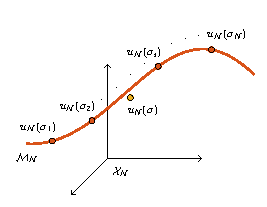
\includegraphics[width=0.6\textwidth]{figures/rb.pdf}
\end{frame}

\begin{frame}[t]
    \frametitle{Intermission: Reduced Basis Method}
    \framesubtitle{Certified error bound}

\end{frame}

\begin{frame}[t]
    \frametitle{Intermission: Reduced Basis Method}
    \framesubtitle{inf-sup-constant}

\end{frame}

\begin{frame}[t]
    \frametitle{Intermission: Reduced Basis Method}
    \framesubtitle{Offline stage}

\end{frame}

\begin{frame}[t]
    \frametitle{Intermission: Reduced Basis Method}
    \framesubtitle{Online stage}

\end{frame}


\begin{frame}[t]
    \frametitle{Reduced basis method}

    \begin{itemize}
        \item Replace the fields $w_A, w_B$ with parametric functions
        \begin{equation}
            w(\bm \sigma) = \sum_{j = 1}^{N} \sigma_{j} \phi_{j},
        \end{equation}
        where $N \in \mathbb{N} \cup \Set{ \infty }$, $\bm \sigma \in [-1, 1]^{N}$ and $\phi_{j} \in L_{\infty}$, $j = 1, \dots, N$.
    \end{itemize}

\end{frame}
